\documentclass{article}

% packages
\usepackage{graphicx}
\usepackage{lastpage}
\usepackage{fancyhdr}
\usepackage[hidelinks]{hyperref}
\usepackage{color}

% page margins
\addtolength{\topmargin}{-0.75in}
\addtolength{\oddsidemargin}{-1.0in}
\addtolength{\evensidemargin}{-1.0in}
\addtolength{\textwidth}{2.0in}
\addtolength{\textheight}{1.5in}

% header and footer
\pagestyle{fancy}
\fancyhf{}
\lhead{Fault-Tolerant Quadcopter}
\rhead{\textit{Vaughn, Mayank, Cooper}}
\cfoot{\thepage\ of \pageref{LastPage}}
\rfoot{\today}

% custom commands
\newcommand{\HREF}[2]{{\color{blue}\underline{\smash{\href{#1}{#2}}}}}

% metadata
\title{ECE 453 Project Proposal}
\author{Vaughn Kottler}
\author{Mayank Katwal}
\author{Cooper Green}

\begin{document}

\begin{center}

	{\huge\textbf{ECE 453 Project Proposal} (Fall 2018)}

	{\large University of Wisconsin-Madison}

	{\large\textit{Vaughn Kottler, Mayank Katwal, Cooper Green}}

\end{center}

\section{Introduction}

We are interested in building a \textit{quadcopter} plus
\textit{ground station} and \textit{web-based user interface}.
We have chosen to call this project the
\textbf{fault-tolerant quadcopter}. This name reveals one of our
stretch goals that will be covered in a future section.

This document serves as the formal proposal to be vetted by the
course instructor,
\HREF{https://directory.engr.wisc.edu/ece/Faculty/Krachey_Joe/}{Joe Krachey}.
We have
\HREF{https://fault-tolerant-quadcopter.readthedocs.io/en/latest/}
{additional documentation in work online} that we plan to keep in
sync with our project's scope and current progress. At the time
of writing it is not yet in a stable state.

This project is designed for three major bodies of work that were
mentioned above but are better captured by Figure
\ref{fig:high-level}:

\begin{figure}[h]
	\centering
	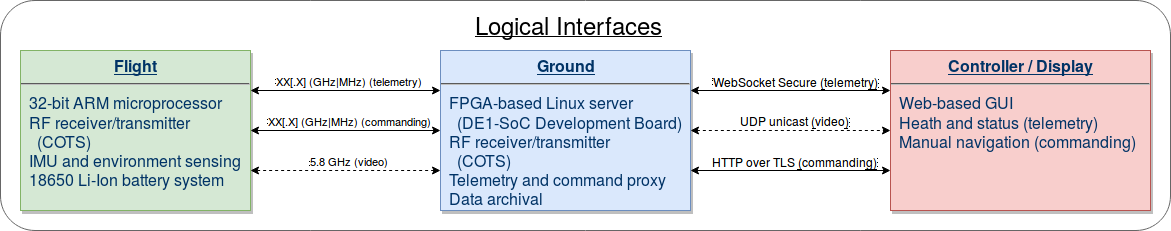
\includegraphics[width=\linewidth]{../src/im/top_level}
	\caption{High-level overview of the major components and
		their interfaces}
	\label{fig:high-level}
\end{figure}

This high-level architecture is inspired by existing aerospace
avionics and software systems that we have done research on
and have some first-hand experience with. Our current, collective
experience with such systems and the technical challenges we
anticipate being associated with them is minimal, though. For
this reason we seek feedback on our lower-level goals and
approach, provided that this high-level idea suffices as
a project worth pursuing.

\section{Technical Features}

TODO

\subsection{Quadcopter}

Responsible Engineer: \textbf{Vaughn}

\begin{figure}[h]
	\centering
	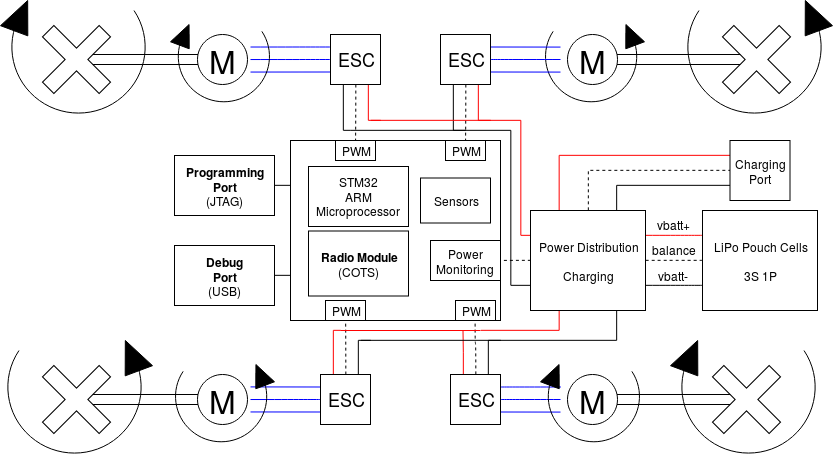
\includegraphics[width=\linewidth]{../src/im/quadcopter}
	\caption{Block diagram view of the quadcopter}
\end{figure}

\begin{itemize}
	\item TODO
\end{itemize}

\subsection{Ground Station}

Responsible Engineer: \textbf{Cooper}

\begin{figure}[h]
	\centering
	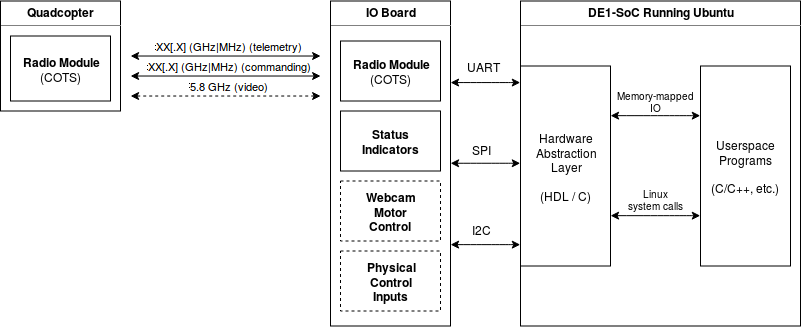
\includegraphics[width=\linewidth]{../src/im/ground_station}
	\caption{Block diagram view of the ground station}
\end{figure}

\begin{itemize}
	\item TODO
\end{itemize}

\subsection{Display and Controller}

Responsible Engineer: \textbf{Mayank}

\begin{figure}[h]
	\centering
	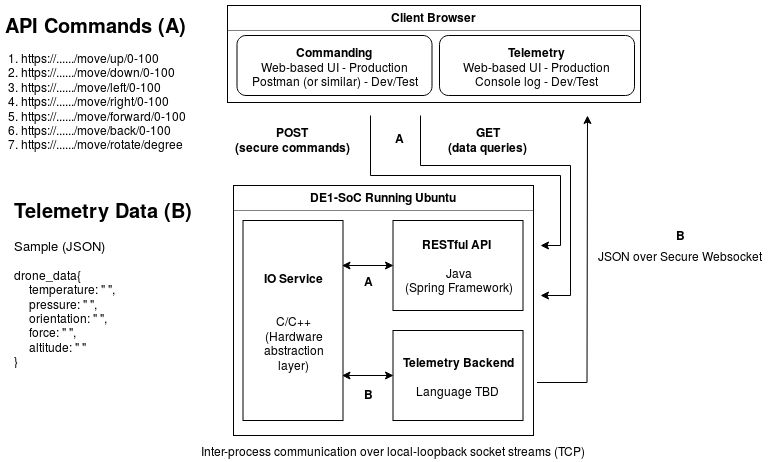
\includegraphics[width=\linewidth]{../src/im/display_controller}
	\caption{Block diagram view of the display and control user
		interface}
\end{figure}

\begin{itemize}
	\item TODO
\end{itemize}

\section{Responsibilities}

How we plan to share responsibility.

\subsection{Vaughn Kottler}

\textbf{Responsible Engineer} for the following:

\begin{description}
	\item [Flight Vehicle] TODO
	\item [Control Algorithms] TODO
\end{description}

\subsection{Mayank Katwal}

\textbf{Responsible Engineer} for the following:

\begin{description}
	\item [Telemetry Display] TODO
	\item [Vehicle Controller] Hardware of Software
\end{description}

\subsection{Cooper Green}

\textbf{Responsible Engineer} for the following:

\begin{description}
	\item [Ground Station] TODO
	\item [Radio Frequency Communication] TODO
\end{description}

\section{Project Management}

TODO

\end{document}
